\documentclass[]{beamer}
\mode<presentation>
% Time-stamp: <2018-08-29 13:45:51 (jonahm)>

% beamer stuff
% Gives us the bottom line with all the goodies
\useoutertheme{infolines}
% Just the theme to use. Should be built into bemaer. Setting the
% height gets rid of a whole lot of whitespace
\usetheme[height=7mm]{Rochester}
\usefonttheme{serif}
% Usually beamer gives you navigation hyperlinks on the bottom
% right. I turned this off. It's annoying.
\setbeamertemplate{navigation symbols}{} 
% Makes my text boxes look pretty
\setbeamertemplate{blocks}[rounded][shadow=true] 
% Makes my bullet points 3d balls
\setbeamertemplate{items}[ball]

% Josh's packages
\usepackage{multimedia}
\usepackage{tabularx}
\usepackage{booktabs}
\usepackage{subfigure}
\usepackage{graphicx}
\usepackage{amsmath}
\usepackage{latexsym}
\usepackage{mathrsfs}

% Packages for me
\usepackage{amsmath,amssymb,latexsym}
\usepackage[mathscr]{eucal}
\usepackage{mathrsfs}
\usepackage{verbatim}
\usepackage{braket}
\usepackage{listings}
\usepackage{amsthm}
\usepackage{xcolor}
%\usepackage[usenames,dvipsnames,svgnames,table]{xcolor}
\usepackage{fancybox}
\usepackage{animate}
% \usepackage{media9}
\usepackage{multicol}
\usepackage{mdframed}
%\usepackage{scalerel}
\usepackage{hyperref}

% Macros

%Blackboard Bold
\newcommand{\R}{\mathbb{R}}
\newcommand{\Z}{\mathbb{Z}}
\newcommand{\N}{\mathbb{N}}
\newcommand{\Q}{\mathbb{Q}}
\newcommand{\A}{\mathbb{A}}
\newcommand{\E}{\mathbb{E}}
% other
\newcommand{\eval}{\biggr\rvert} %evaluated at
\newcommand{\myvec}[1]{\mathbf{#1}} % vectors for me
% total derivatives 
\newcommand{\diff}[2]{\frac{d #1}{d #2}} 
\newcommand{\dd}[1]{\frac{d}{d #1}}
% partial derivatives
\newcommand{\pd}[2]{\frac{\partial #1}{\partial #2}} 
\newcommand{\pdd}[1]{\frac{\partial}{\partial #1}} 
% Order operator
\DeclareRobustCommand{\orderof}{\ensuremath{\mathcal{O}}}

% tikz
\usepackage{tikz}
\usetikzlibrary{arrows}
\usepackage{pgfplots}


% Keys to support piece-wise uncovering of elements in TikZ pictures:
% \node[visible on=<2->](foo){Foo}
% \node[visible on=<{2,4}>](bar){Bar}   % put braces around comma expressions
% 
% Internally works by setting opacity=0 when invisible, which has the 
% adavantage (compared to \node<2->(foo){Foo} that the node is always there, hence
% always consumes space plus that coordinate (foo) is always available.
% 
% The actual command that implements the invisibility can be overriden
% by altering the style invisible. For instance \tikzsset{invisible/.style={opacity=0.2}}
% would dim the "invisible" parts. Alternatively, the color might be set to white, if the
% output driver does not support transparencies (e.g., PS) 
% 
\tikzset{
  invisible/.style={opacity=0},
  visible on/.style={alt={#1{}{invisible}}},
  alt/.code args={<#1>#2#3}{%
    \alt<#1>{\pgfkeysalso{#2}}{\pgfkeysalso{#3}} % \pgfkeysalso doesn't change the path
  },
}

% some nice flowchart features
\tikzset{
    mynode/.style={rectangle,rounded corners,draw=black, top color=white, bottom color=yellow!50,very thick, inner sep=1em, minimum size=3em, text centered},
    myarrow/.style={->, >=latex', shorten >=1pt, thick},
    mylabel/.style={text width=7em, text centered} 
}  

% define a really nice visible "purple"
\definecolor{gimppurple}{HTML}{AD26FB}
% a light grey
\definecolor{lightgrey}{HTML}{E0E0E0}
% for highlighting
\definecolor{deepblue}{rgb}{0,0,0.5}
\definecolor{deepred}{rgb}{0.6,0,0}
\definecolor{deepgreen}{rgb}{0,0.5,0}

% fonts
% Default fixed font does not support bold face
\DeclareFixedFont{\ttb}{T1}{txtt}{bx}{n}{10} % for bold
\DeclareFixedFont{\ttm}{T1}{txtt}{m}{n}{10}  % for normal

% Python style for highlighting
\newcommand\pythonstyle{\lstset{
language=Python,
basicstyle=\footnotesize\ttm,
otherkeywords={self},
keywordstyle=\ttb\color{deepblue},
emph={__init__},           
emphstyle=\ttb\color{deepred},
commentstyle=\ttfamily\color{deepred},
stringstyle=\color{deepgreen},
frame=tb,                     
showstringspaces=false        
}}

% Python environment
\lstnewenvironment{python}[1][]
{
\pythonstyle
\lstset{#1}
}
{}

\newcommand{\backupbegin}{
   \newcounter{finalframe}
   \setcounter{finalframe}{\value{framenumber}}
}
\newcommand{\backupend}{
   \setcounter{framenumber}{\value{finalframe}}
}

% a macro for a useful transition slide
\newcommand{\transitionslide}[1]{
  \begin{frame}[plain]
  \vfill
  \centering
  \begin{beamercolorbox}[sep=8pt,center,shadow=true,rounded=true]{title}
    \usebeamerfont{title}{#1}
  \end{beamercolorbox}
  \vfill
\end{frame}
}

\title[Visualization]{Visualization of Simulation Data}
\author[J. Miller]{Jonah M. Miller}
\institute[LANL]{\color{blue}Los Alamos National Lab}

\date[ET Workshop]{\color{black}European Einstein Toolkit Workshop\\September, 2018}

\begin{document}

\begin{frame}[plain]
\titlepage
\end{frame}

\begin{frame}
  \frametitle{Why Visualize in 3D?}
  \begin{columns}
    \begin{column}{6cm}
      \begin{itemize}
      \item Eye catching---great for journals, posters, talks, etc.
      \item 3D structures not visible in slice plots can be visible in
        3D volume renders
      \item Useful for exploring and understanding your own data
      \end{itemize}
    \end{column}
    \begin{column}{6cm}
      \begin{center}
        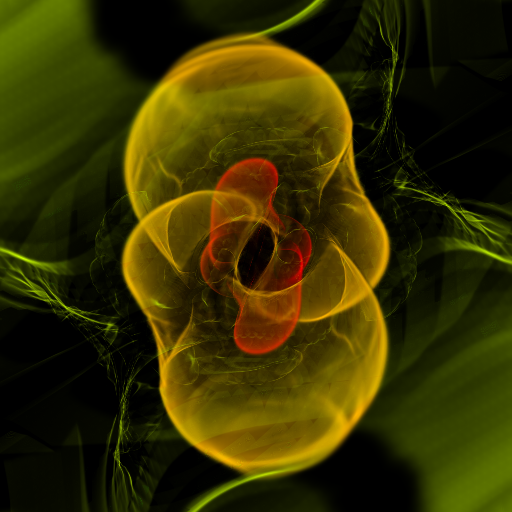
\includegraphics[width=5.5cm]{figures/psi4r-it-1024/psi4r-iteration-1024-volume-f-32}
        %\animategraphics[width=5.5cm,every=1,autoplay,loop]{6}{figures/psi4r-it-1024/psi4r-iteration-1024-volume-f-}{00}{32}
      \end{center}
    \end{column}
  \end{columns}
\end{frame}

\begin{frame}
  \frametitle{What You Will Learn}
  \begin{enumerate}
  \item (Very roughly) how does volume rendering work?
  \item How to put your simulation data into these tools
    \begin{itemize}
    \item Your code has one representation of the physics, the data
      file has another, the visualization tool yet another.
    \item Mapping these representations into each other can be hard.
    \item We'll do it for:
      \begin{itemize}
      \item  Einstein Toolkit data
      \item  Arbitrary simulation data
      \end{itemize}
    \end{itemize}
  \item Some tips and tricks
    \begin{itemize}
    \item Visualization best practices
    \item Idiosyncracies of each tool
    \end{itemize}
  \end{enumerate}
\end{frame}

\begin{frame}
  \frametitle{Volume Rendering and Ray Tracing}
  \resizebox{12cm}{!}{
    \begin{tikzpicture}
      \node[inner sep=0pt] at (0,0) {
        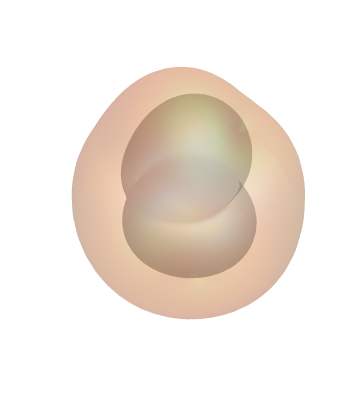
\includegraphics[width=4cm,height=4cm,clip,trim={1cm 1cm 1cm 1cm}]{figures/blob-rand-ylm}
      };
      % plane
      \filldraw[draw=black,thick,fill=red!20,opacity=0.75]
      (-4.5,-2,-2) -- (-4.5,-2,2)
      -- (-4.5,2,2) -- (-4.5,2,-2)
      -- cycle;
      \draw[black] (-4.5,0.6) ellipse(0.35 and 0.75);
      \draw[black] (-4.5,-0.6) ellipse(0.35 and 0.75);
      % source
      %\shadedraw[ball color=blue] (5.,0) circle (1.2);
      % right
      \draw[ultra thick,<-] (2,1) -- (4,1);
      \draw[ultra thick,<-] (2,0) -- (4,0);
      \draw[ultra thick,<-] (2,-1) -- (4,-1);
      % left
      \draw[ultra thick,->] (-2,1) -- (-4,1);
      \draw[ultra thick,->] (-2,0) -- (-4,0);
      \draw[ultra thick,->] (-2,-1) -- (-4,-1);
      % labels
      \draw (-4.5,-3) node[below] {Screen/Eyes};
      \draw (0,-3) node[below] {Data/Transfer Function};
      \draw (4,-3) node[below] {Source};
    \end{tikzpicture}
  }
\end{frame}

\begin{frame}
  \frametitle{What do we care about in a simulation?}
  \begin{tikzpicture}
    \draw[ultra thick,->] (7,3) -- (4,1.5);
    \node[inner sep=0pt] at (2,2) {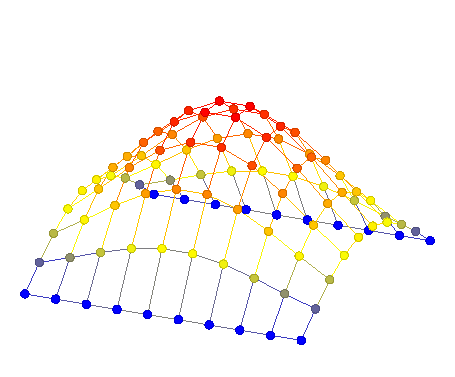
\includegraphics[width=4cm,trim={0cm 0cm 0cm 0cm},clip]{figures/surface-scatter-small}};
    \node[inner sep=0pt] at (9,3.5) {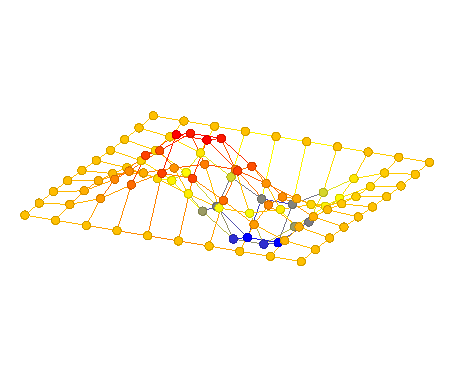
\includegraphics[width=8cm,trim={0cm 0cm 0cm 0cm},clip]{figures/surface-scatter}};
    \draw[ultra thick,->] (5,7) -- (7,4);
    \node[inner sep=0pt] at (4,6) {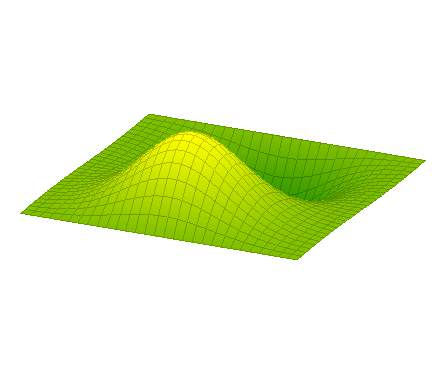
\includegraphics[width=8cm,trim={0.5cm 0cm 0cm 1.75cm},clip]{figures/surface-smooth}};
  \end{tikzpicture}
\end{frame}

\begin{frame}
  \frametitle{What do we care about in a simulation?}
  \begin{center}
    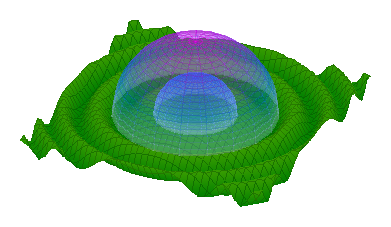
\includegraphics[width=12cm]{figures/wavey}
  \end{center}
\end{frame}

\begin{frame}
  \frametitle{What do we care about in a simulation?}
    \begin{center}
    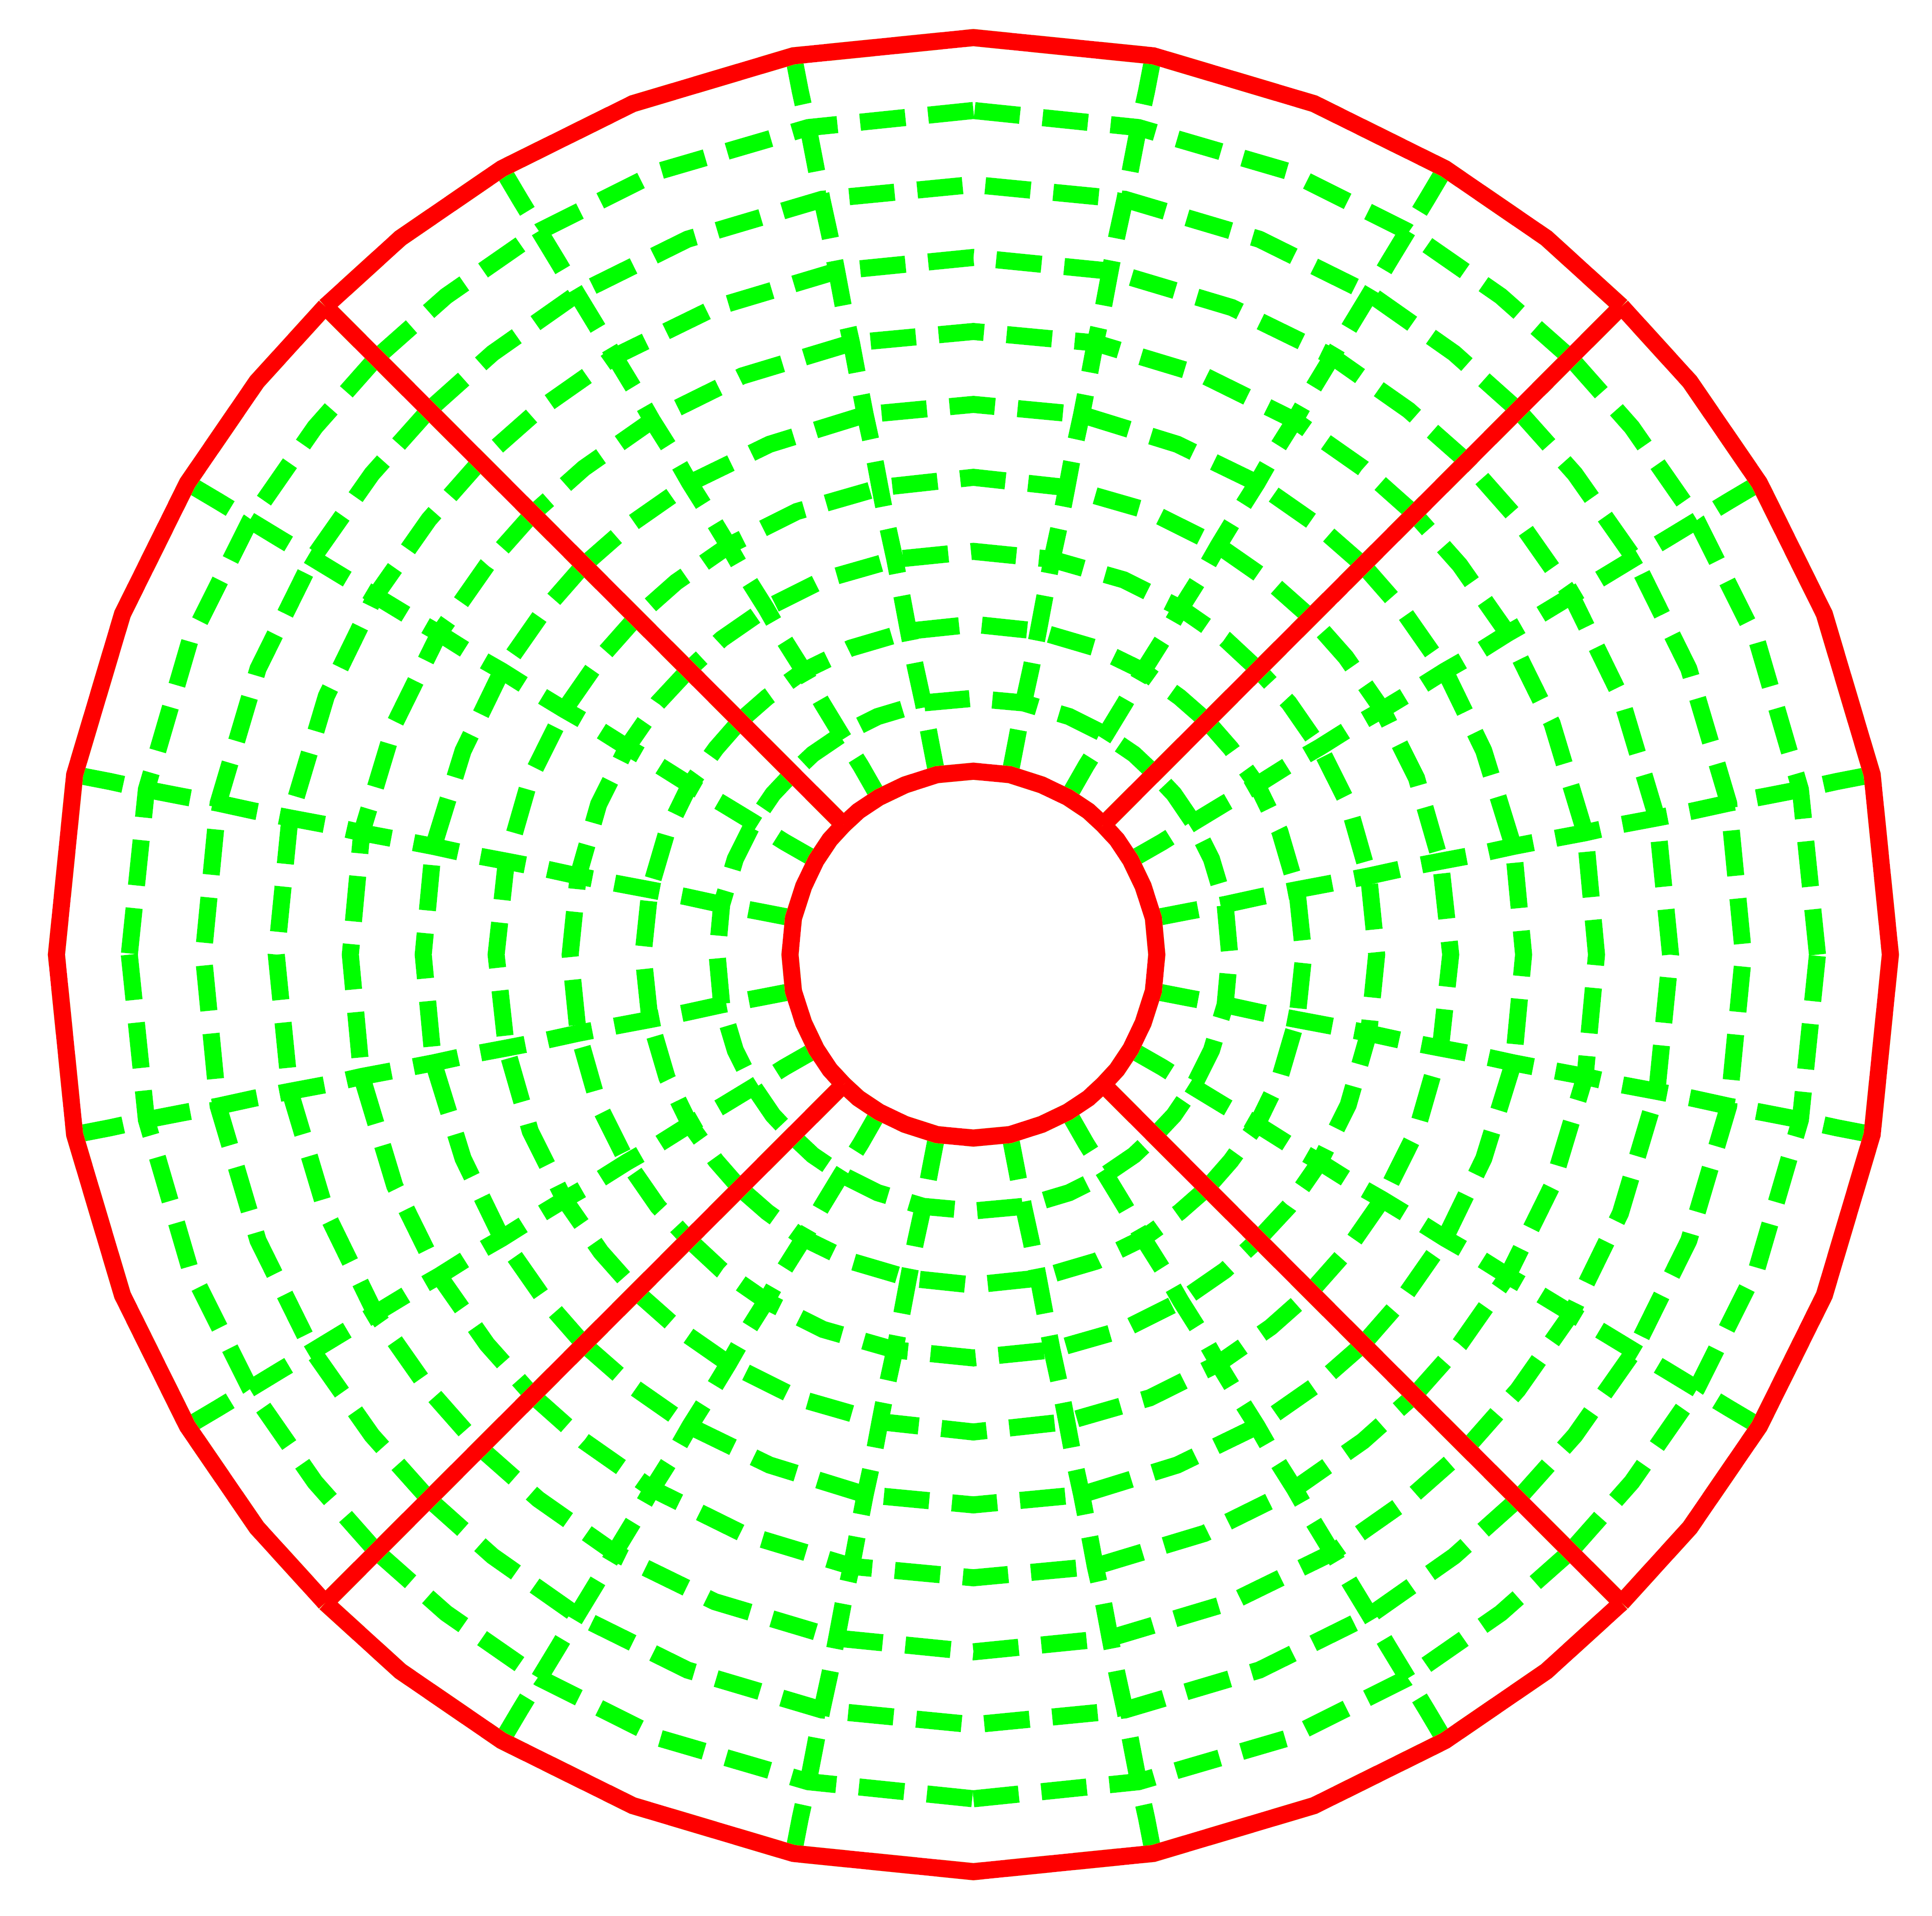
\includegraphics[width=5.5cm]{figures/fourpatches.png}
    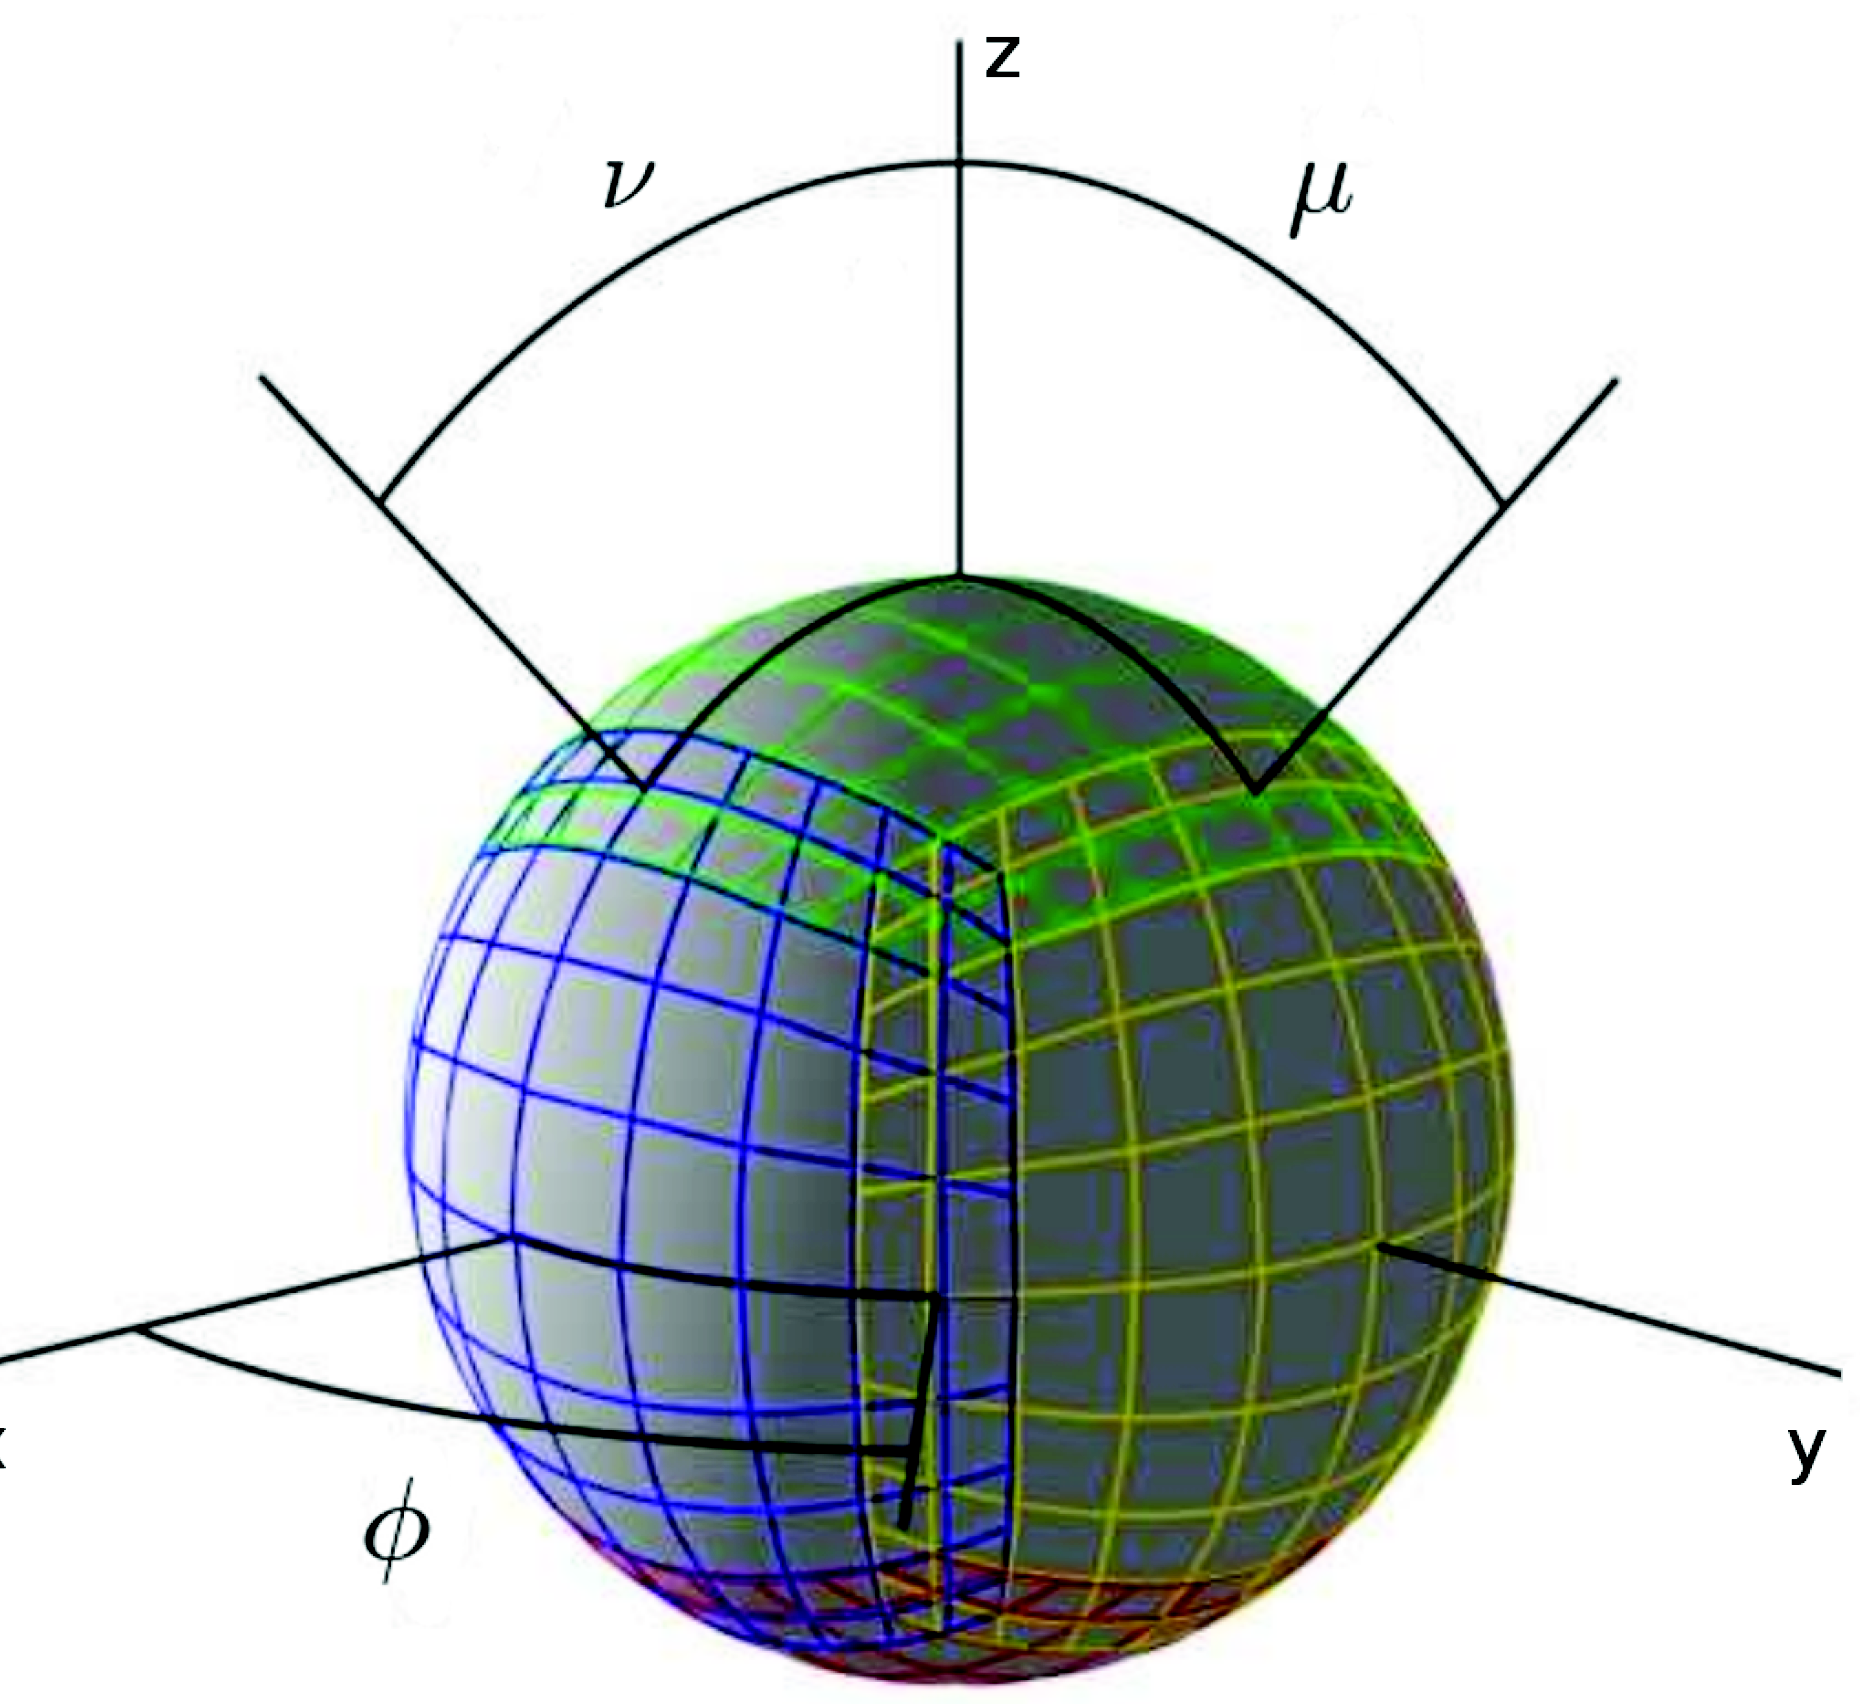
\includegraphics[width=5.5cm]{figures/sixpatches.png}
  \end{center}
  Schnetter \textit{et al} 2006 Class. \textit{Quantum Grav.} \textbf{23} S553\\
  Pollney \textit{et al} 2011 \textit{Phys. Rev. D} \textbf{83} 044045
\end{frame}


\begin{frame}
  \frametitle{Visualization Tools}
  \begin{columns}
    \begin{column}{6cm}
      \begin{center}
        
\includegraphics[width=0.9\columnwidth]{figures/python-logo-master-v3-TM}
      \end{center}
    \end{column}
    \begin{column}{6cm}
      \begin{itemize}
      \item \textbf{\color{green}Pros:} Simple. Easy to explore/inspect data.
      \item \textbf{\color{red}Cons:} Limited. 3D visualization hard.
      \end{itemize}
    \end{column}
  \end{columns}
  \noindent\rule{\textwidth}{1pt}
  \begin{columns}
    \begin{column}{6cm}
      \begin{center}
        
\includegraphics[width=0.35\columnwidth]{figures/VisItLogoTrans}
        
\includegraphics[width=0.55\columnwidth]{figures/ParaView_Logo}
      \end{center}
    \end{column}
    \begin{column}{6cm}
      \begin{itemize}
      \item \textbf{\color{green}Pros:} Very flexible. Contain graphical UI.
      \item \textbf{\color{red}Cons:} Opaque. Hard to use in parallel.
      \end{itemize}
    \end{column}
  \end{columns}
  \noindent\rule{\textwidth}{1pt}
  \begin{columns}
    \begin{column}{6cm}
      \begin{center}
        
\includegraphics[width=0.4\columnwidth]{figures/yt_logo}
      \end{center}
    \end{column}
    \begin{column}{6cm}
      \begin{itemize}
      \item \textbf{\color{green}Pros:} Incorporates meaningful
        physics and analysis. Hack able. Parallel.
      \item \textbf{\color{red}Cons:} Less flexible. No interactive UI.
      \end{itemize}
    \end{column}
  \end{columns}
\end{frame}

\begin{frame}[fragile]
  \frametitle{Exercise: Inspecting Arbitrary Data in Python}
\begin{python}
import h5py
import numpy as np
data = {}
with h5py.File('harmdisk2d/data.h5','r') as f:
    for k,v in f.items():
        data[k] = v.value
\end{python}
  \begin{center}
    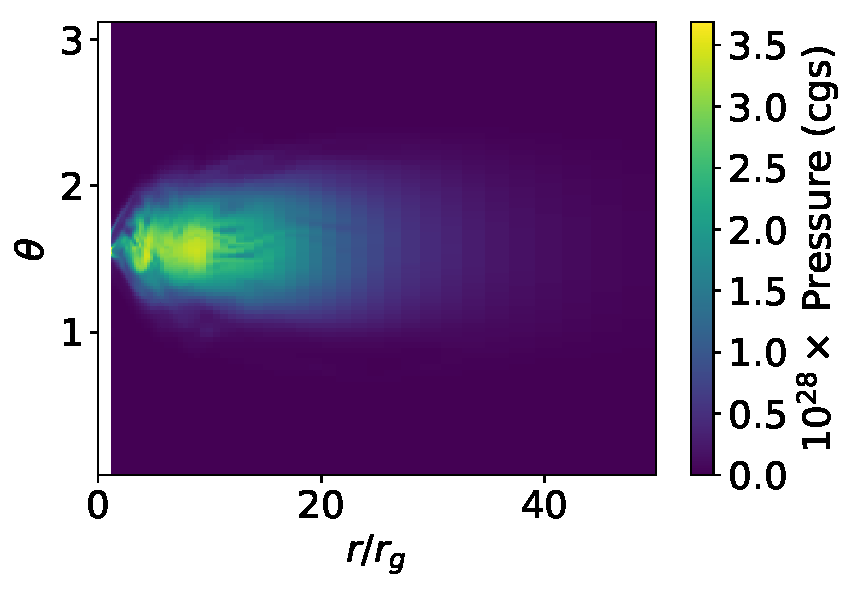
\includegraphics[height=4cm]{figures/harmdisk2d}
  \end{center}
\end{frame}

\begin{frame}[fragile]
  \frametitle{Exercise: Inspecting Carpet AMR Data in Python}

\end{frame}

\begin{frame}
  \frametitle{Important Carpet AMR Concepts}
    \resizebox{12cm}{!}{
    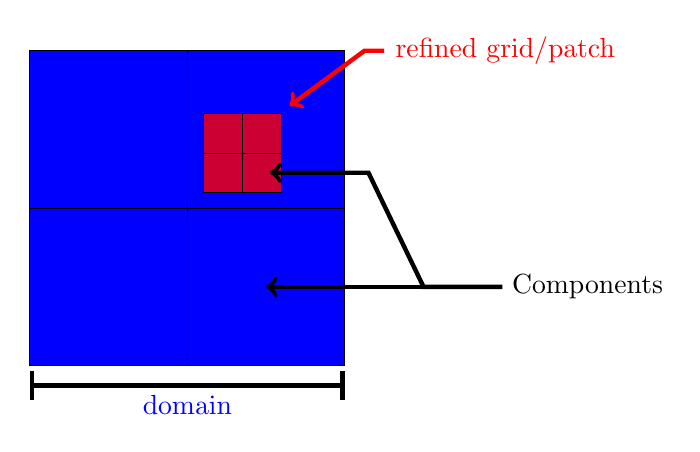
\begin{tikzpicture}
      \filldraw[blue] (0,0) rectangle (4,4);
      \draw (0,0) rectangle (2,2);
      \draw (2,2) rectangle (4,4);
      \draw (0,2) rectangle (2,4);
      \draw (2,0) rectangle (4,2);
      \draw[ultra thick,black,|-|] (0,-0.25) -- (4,-0.25);
      \draw (2,-0.25) node[below] {\color{blue}domain};
      \filldraw[red,opacity=0.8] (2.2,2.2) rectangle (3.2,3.2);
      \draw[ultra thick,red,<-] (3.3,3.3)
      -- (4.25,4.) -- (4.5,4) node[right] {\color{red}refined grid/patch};
      \draw (2.2,2.2) rectangle ++(0.5,0.5);%(2.5,2.5);
      \draw (2.7,2.7) rectangle ++(0.5,0.5);%(3,3);
      \draw (2.2,2.7) rectangle ++(0.5,0.5);%(2.5,3);
      \draw (2.7,2.2) rectangle ++(0.5,0.5);%(3,2.5);

      \coordinate (cmp) at (6,1);
      \coordinate (knk) at (5,1);

      \draw (cmp) node[right] {\color{black}Components};
      \draw[ultra thick,black,<-] (3.05,2.45) -- (4.3,2.45) -- (knk) -- (cmp);
      \draw[ultra thick,black,<-] (3,1) -- (knk);
    \end{tikzpicture}
  }
\end{frame}

\end{document}